\section{Gangbild Anpassungen}
Das natürlich erlernte Gangbild eines gesunden Menschen ist sehr komplex. Im folgenden Kapitel wird das Gangbild des Mixamo Charakters basierend auf den Gangphasen der menschlichen Fortbewegung analysiert und angepasst. Diese Gangphasen umfassen verschiedene Stadien der Fortbewegung, wie das Abstoßen, das Schwingen des Beins und den Fersenauftritt, die zusammen ein fließendes und ausgewogenes Gehen ermöglichen. Wie bereits in der Analyse der Walker Demo erwähnt, ist das Gangbild des Walker Demo Läufers menschenähnlich und für die vereinfachte Darstellung des Charakters durchaus ausreichend. Die gesteigerte Komplexität des 3D-Modells beim Mixamo Charakter führt bei der Wahrnehmung zu einem gesteigerten Realismus. Der Mixamo Charakter lernt zudem eher ein Galoppieren als das Laufen, welches der Walker Demo Läufer nach dem Training aufweist. Durch den gesteigerten Realismus und die Verschlechterung des Gangbilds wird im folgenden Kapitel untersucht, wie zusätzliche Belohnungen das erlernte Gangbild beeinflussen können. Dabei werden gezielt Belohnungen eingeführt, die darauf abzielen, das Gesamterscheinungsbild der Fortbewegung zu verbessern.

\subsection{Beinwechsel}
Das menschliche Gangbild besteht aus sich wiederholenden Phasen, die abwechselnd bei beiden Beinen durchlaufen werden. Um den Läufer dazu zu motivieren, in einem regelmäßigen Intervall das vorangehende Bein zu wechseln, wird ein Timer eingeführt, der von 0 startet, sobald das vorderste Bein in Zielrichtung gewechselt wurde. Ausgehend von der verstrichenen Zeit seit dem letzten Wechsel erhält der Läufer dann eine Strafe. Wie in Abbildung \ref{fig:plot_beinwechsel} zu sehen ist, bleibt die Bestrafung bis 1,2 Sekunden bei 0. Bleibt ein Bein länger als 1,2 Sekunden vorne, steigt die Bestrafung linear an, bis sie bei 5,2 Sekunden das Maximum von -1 erreicht. Initial wurde ein Schwellenwert für die Bestrafung von 2 Sekunden von einem ähnlichen Projekt aus dem Youtube Video \grqq{}AI Learns to Walk (deep reinforcement learning)\grqq{} übernommen.\cite{aiwarehouse} Nach dem Training war jedoch deutlich zu sehen, dass eine Beinwechselperiode von 2 Sekunden zu lang ist. Durch eigene Experimente des Verfassers wurde eine durchschnittliche Beinwechselzeit von 1,2 Sekunden ermittelt. Für die Bestimmung dieses Wertes wurden Videoaufnahmen des Gehens erstellt, anhand derer anschließend die Dauer eines Beinwechsels festgelegt werden konnte.

\begin{figure}[H]
  \centering
  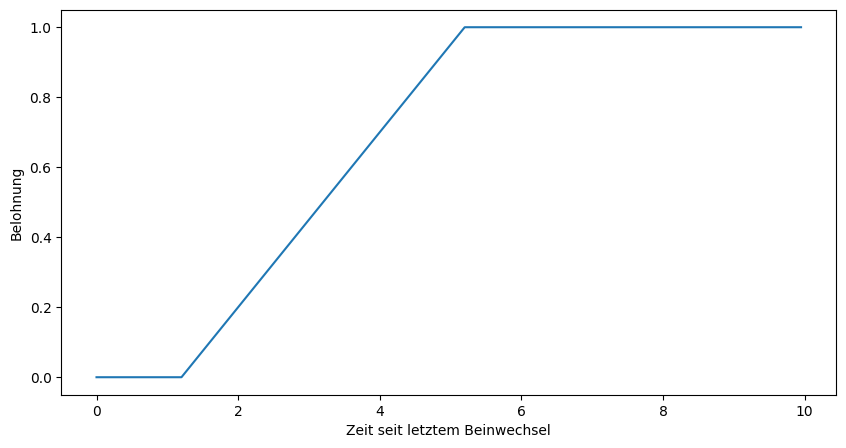
\includegraphics[width=0.9\textwidth]{img/plot_beinwechsel} 
  \caption{Beinwechsel Belohnung}
  \label{fig:plot_beinwechsel}
\end{figure}

Das Einführen dieser Bestrafung hat beim Training erfolgreich dazu geführt, dass der Läufer in regelmäßigen Abständen das Standbein wechselt (siehe Abbildung \ref{fig:mixamo_versuch11_gangbild}). Diese Anpassung führte zu einer spürbaren Verbesserung der Bewegungsdynamik des Läufers, insbesondere in Bezug auf die Regelmäßigkeit der Schritte. Es wird das Verharren in einer Position verhindert, was das galoppieren bestraft, und so zu einer flüssigeren und natürlicheren Fortbewegung führt.

\begin{figure}[H]
  \centering
  \begin{tabular}{ccc}
    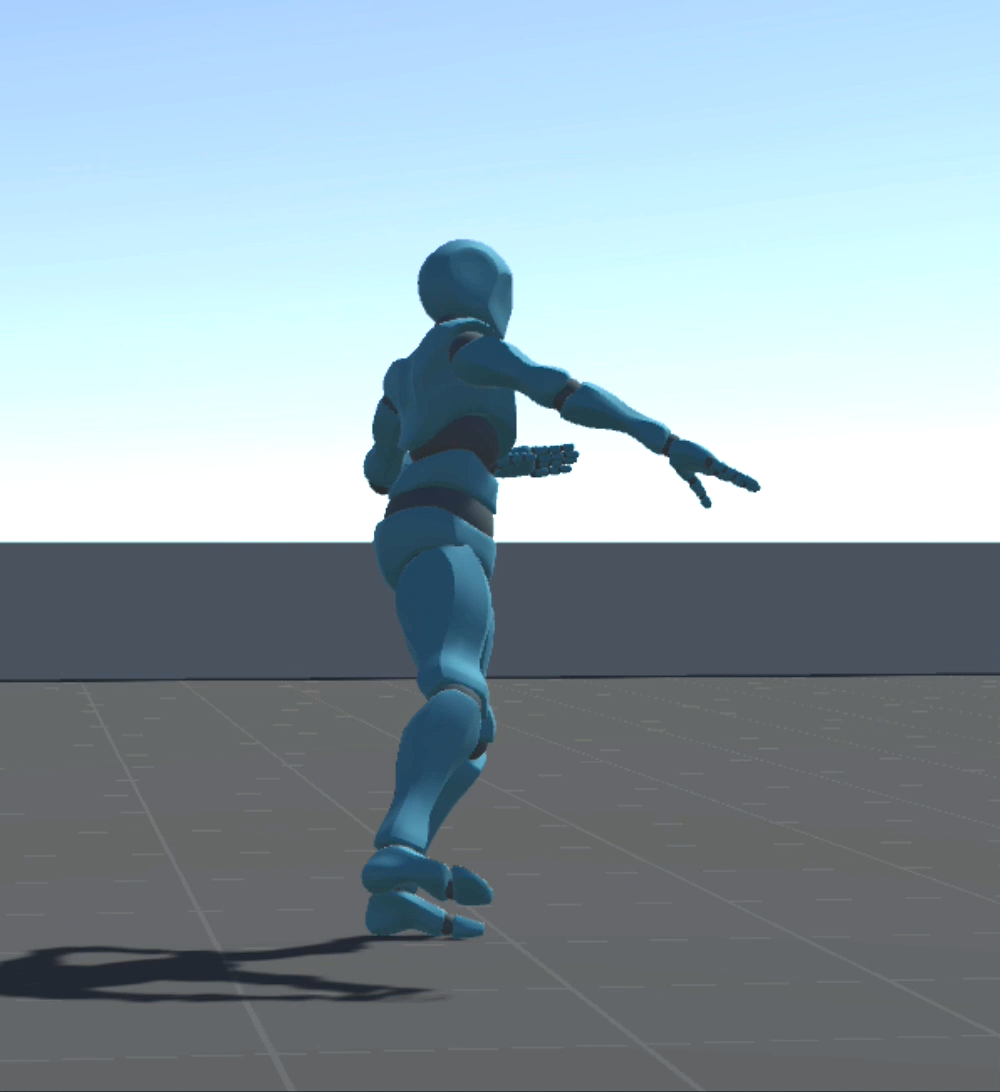
\includegraphics[width=0.27\textwidth]{img/charakter_mixamo_laufen1} & 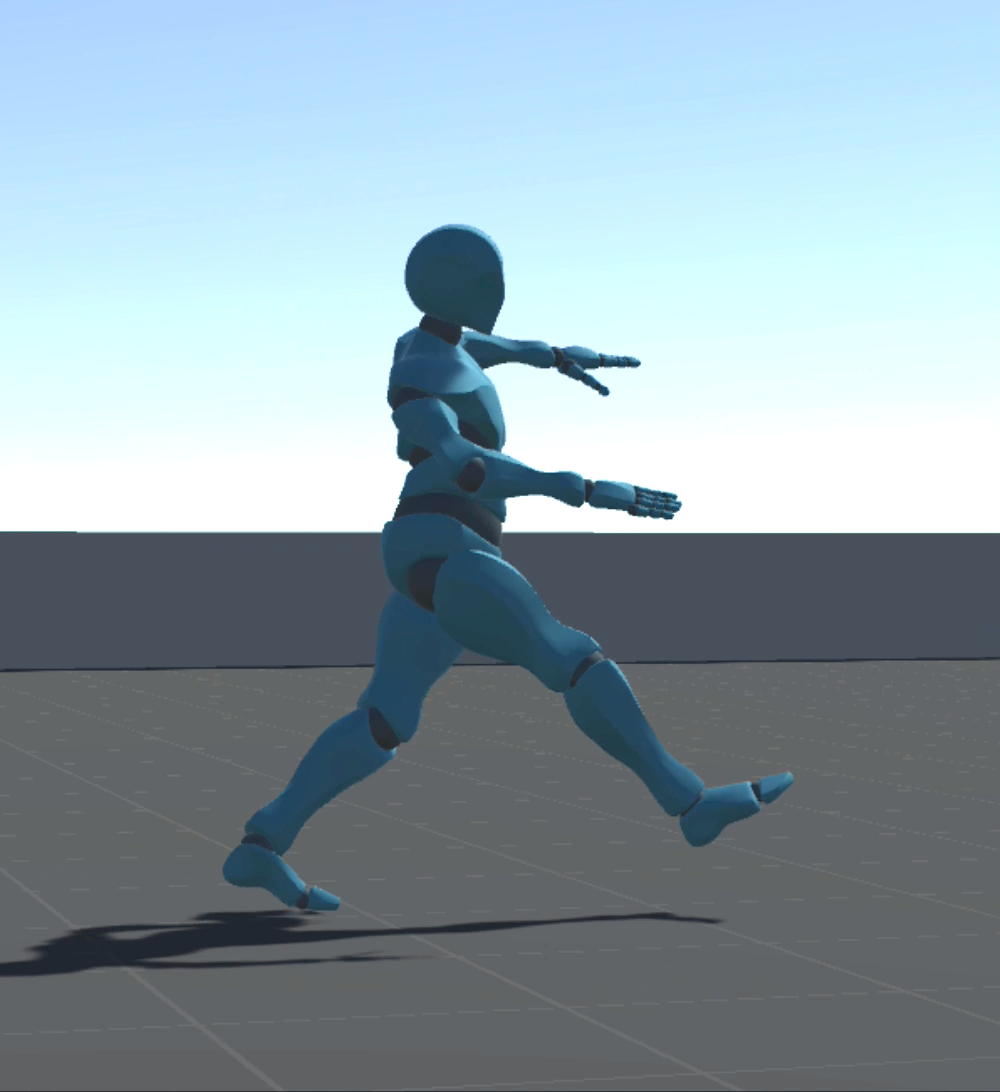
\includegraphics[width=0.27\textwidth]{img/charakter_mixamo_laufen2}  & 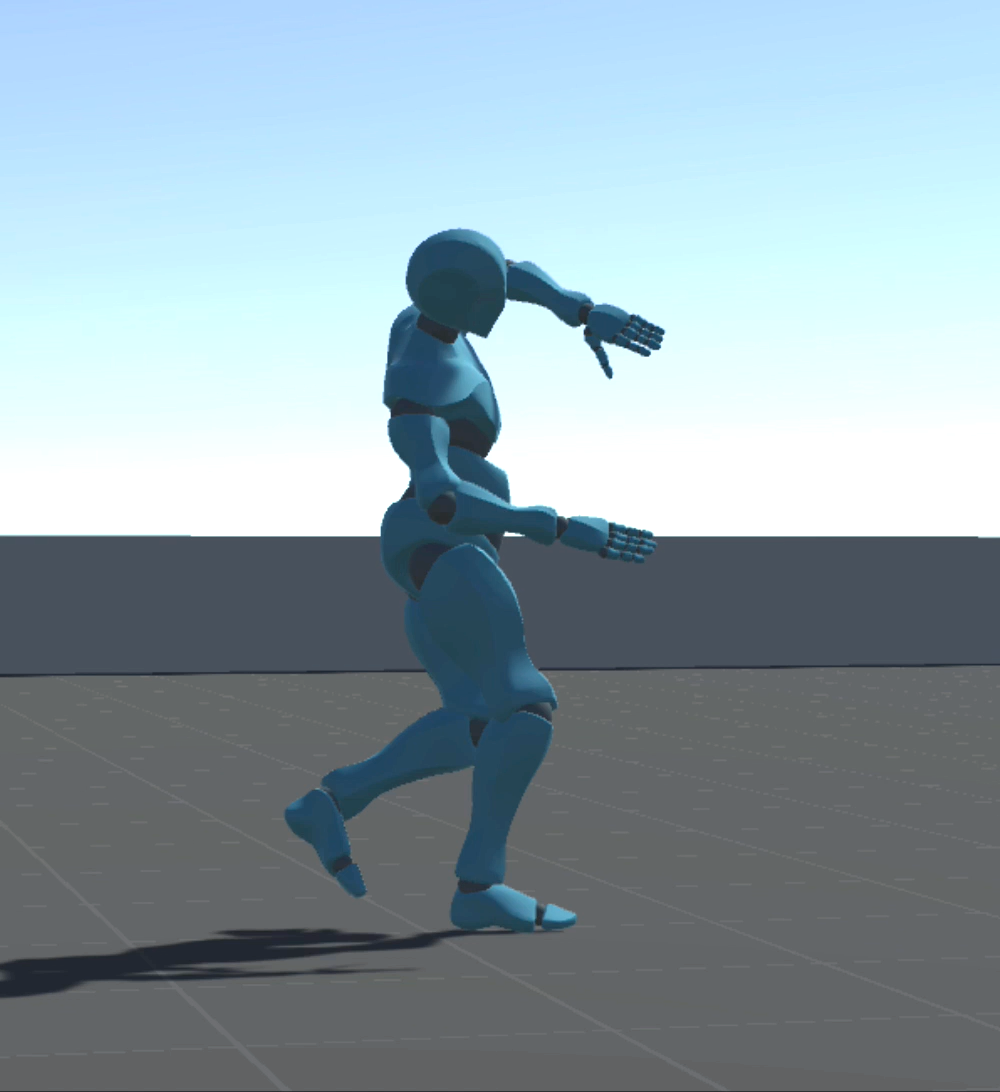
\includegraphics[width=0.27\textwidth]{img/charakter_mixamo_laufen3} \\
    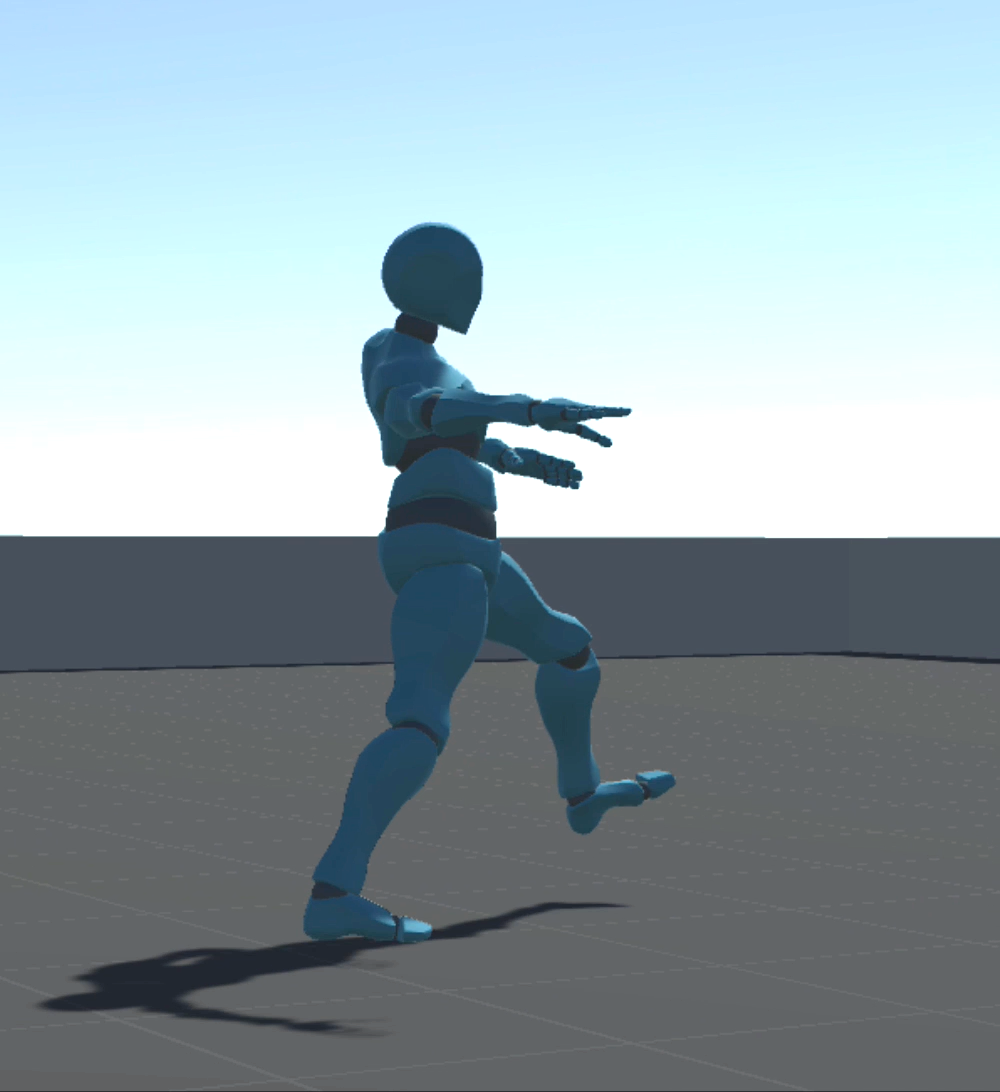
\includegraphics[width=0.27\textwidth]{img/charakter_mixamo_laufen4}  & 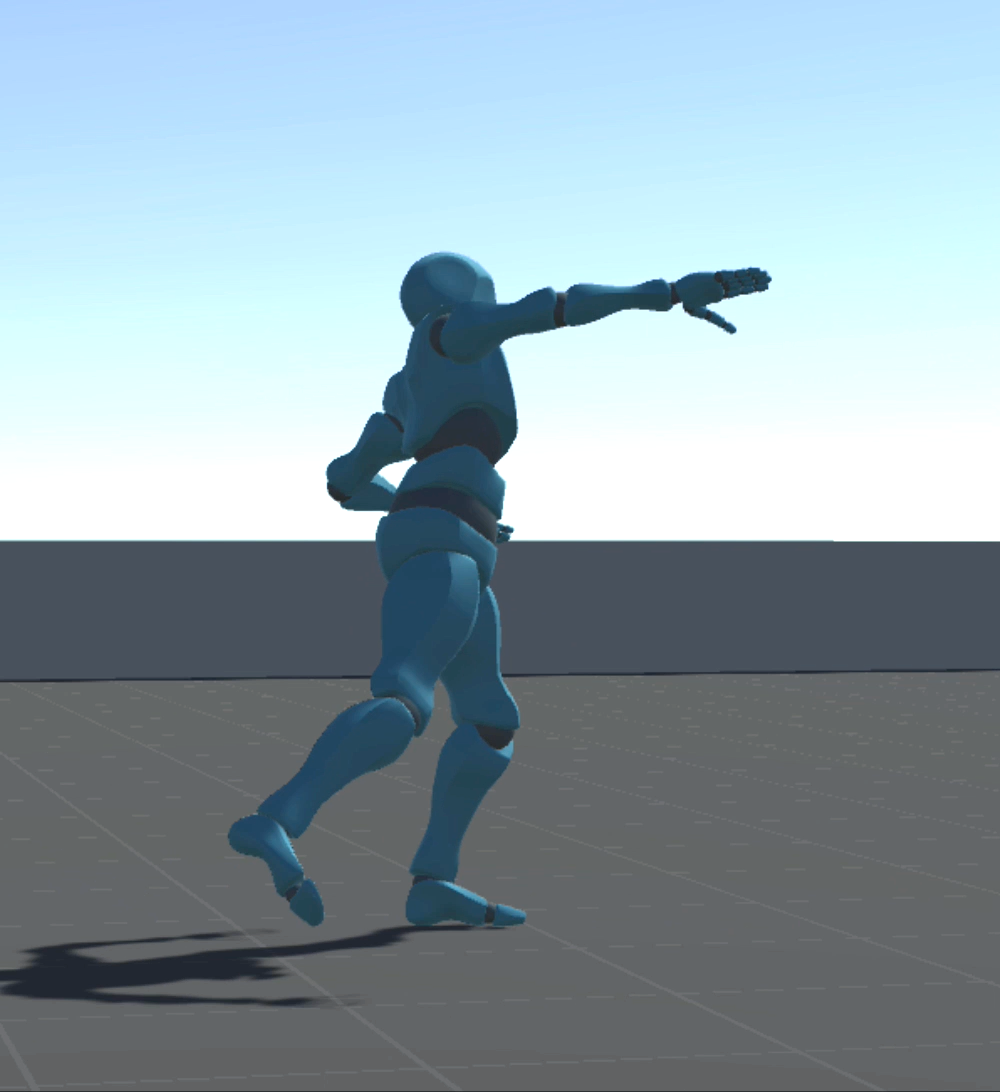
\includegraphics[width=0.27\textwidth]{img/charakter_mixamo_laufen5}  & 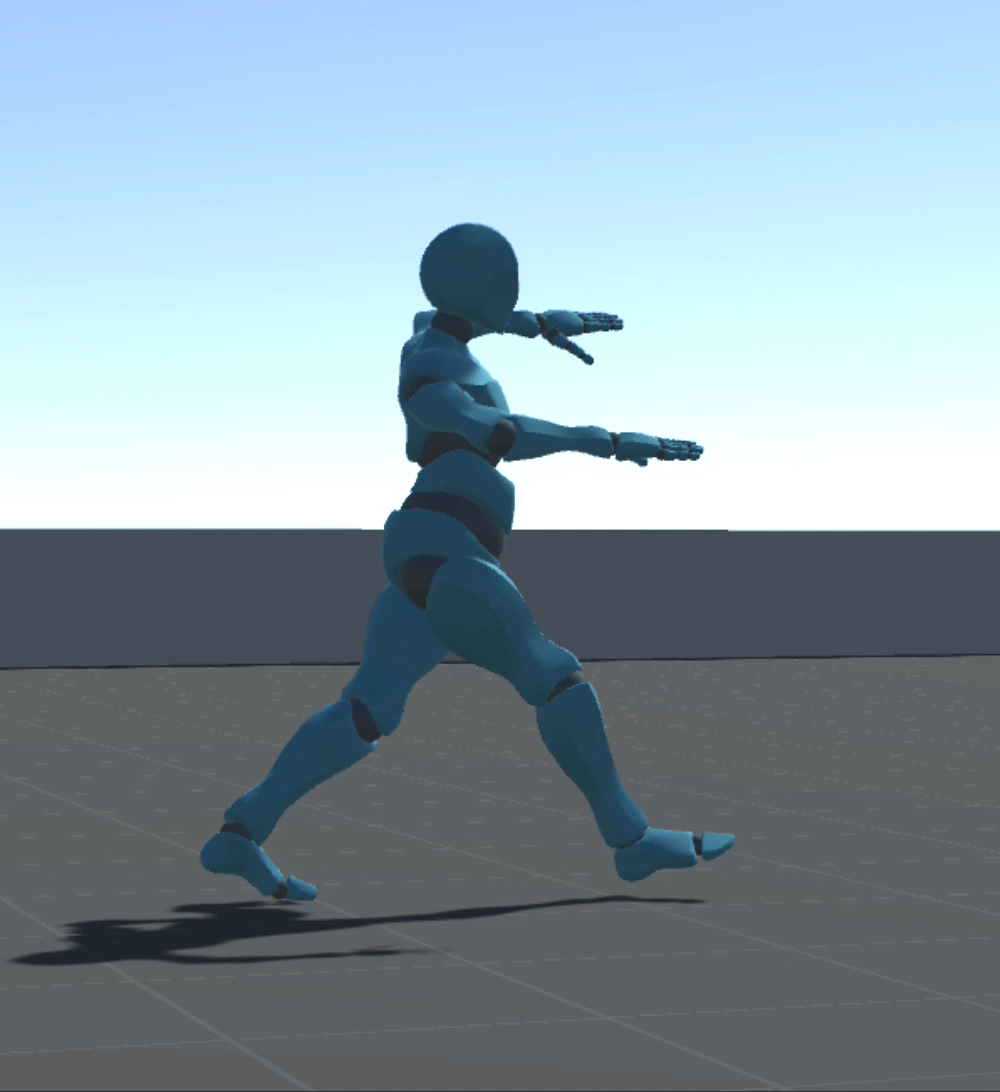
\includegraphics[width=0.27\textwidth]{img/charakter_mixamo_laufen6} \\
  \end{tabular}
  \caption{Mixamo Versuch 11 Gangbild}
  \label{fig:mixamo_versuch11_gangbild}
\end{figure}

\subsection{Energieminimierung}
Ein großer Einfluss auf die Entwicklung des menschlichen Gangbilds ist die Energieminimierung. Der Läufer hat keine Wahrnehmung von Aufwand, daher sind die erlernten Bewegungsabläufe oft alles andere als effizient. Um das Gangbild weiter zu verbessern, wird eine Belohnung eingeführt, die den Agenten dafür belohnt, wenn er so wenig wie möglich Kraft aufwendet, um das Ziel zu erreichen. Genauer gesagt wird er dafür bestraft, wenn die Gelenksteuerung einen zu hohen Energiekonsum aufweist. Ähnlich wie die Fußwechselbestrafung wird auch für die Energieminimierung eine Funktion verwendet, bei der die Bestrafung zwischen 150 und 3150 Watt linear ansteigt. Die Wahl der Energie-Schwellenwerte orientiert sich an den im Artikel \grqq{}Assessing the metabolic cost of walking: The influence of baseline subtractions\grqq{} angegebenen durchschnittlichen Energieaufwänden.\cite{5333126}  Für eine Geschwindigkeit von 0,2 m/s bis 1,9 m/s wird ein Energieaufwand von 2,14 bis 6,90 Watt pro kg festgelegt. Mit einem Gewicht des Läufers von 109 kg ergibt sich ein Bereich von 233 bis 752 Watt bei einer vergleichbaren Effizienz. Dieser Bereich ist weit genug gefasst, sodass der Läufer Belohnungen über 0 erreichen kann. Ergebnisse mit steigender Effizienz führen zu nahezu vernachlässigbaren Bestrafungen. Die Funktion ergibt für 233 Watt eine Bestrafung von 0,027 und für 752 Watt eine Bestrafung von 0,2. Aufgrund der variablen Sensitivität der Geschwindigkeitsbelohnungsfunktion erreicht der Läufer selten eine solch hohe Geschwindigkeit, sodass die Bestrafung durch das Optimieren der Gangbewegung nahezu auf 0 reduziert werden kann.

\begin{figure}[H]
  \centering
  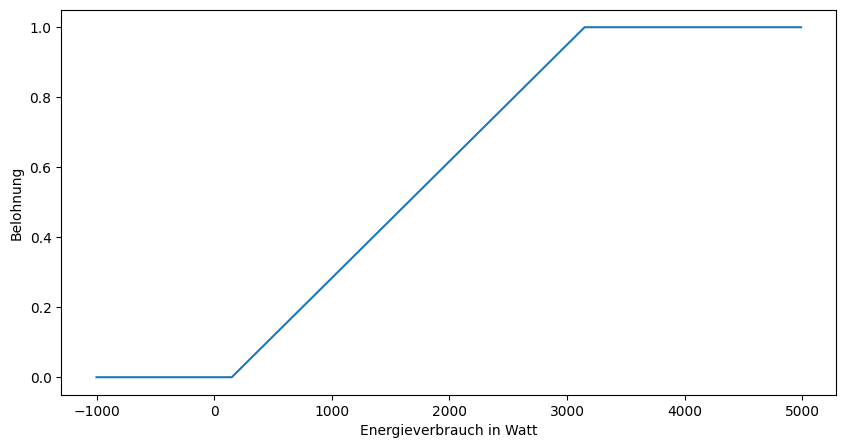
\includegraphics[width=0.9\textwidth]{img/plot_energiespar} 
  \caption{Energiespar Belohnung}
  \label{fig:plot_energiespar}
\end{figure}

Die Energieminimierung bringt den Läufer dazu, seine Bewegungen zu optimieren und somit zu minimieren. Das Gangbild wirkt dadurch natürlicher, insbesondere weil die Bein- und Körperbewegungen wesentlich verbessert wurden. Zuvor hat der Läufer beim Laufen den Oberkörper über das Standbein gekippt, nach der Einführung der Energiesparbelohnung wurde die Oberkörperbewegung minimiert. Allerdings hat die Energieminimierung auch dazu geführt, dass die Arme so gut wie gar nicht mehr bewegt werden. Das Fehlen der Armbewegung tritt im Gesamtbild der natürlichen Bewegung negativ auf.

\begin{figure}[H]
  \centering
  \begin{tabular}{ccc}
    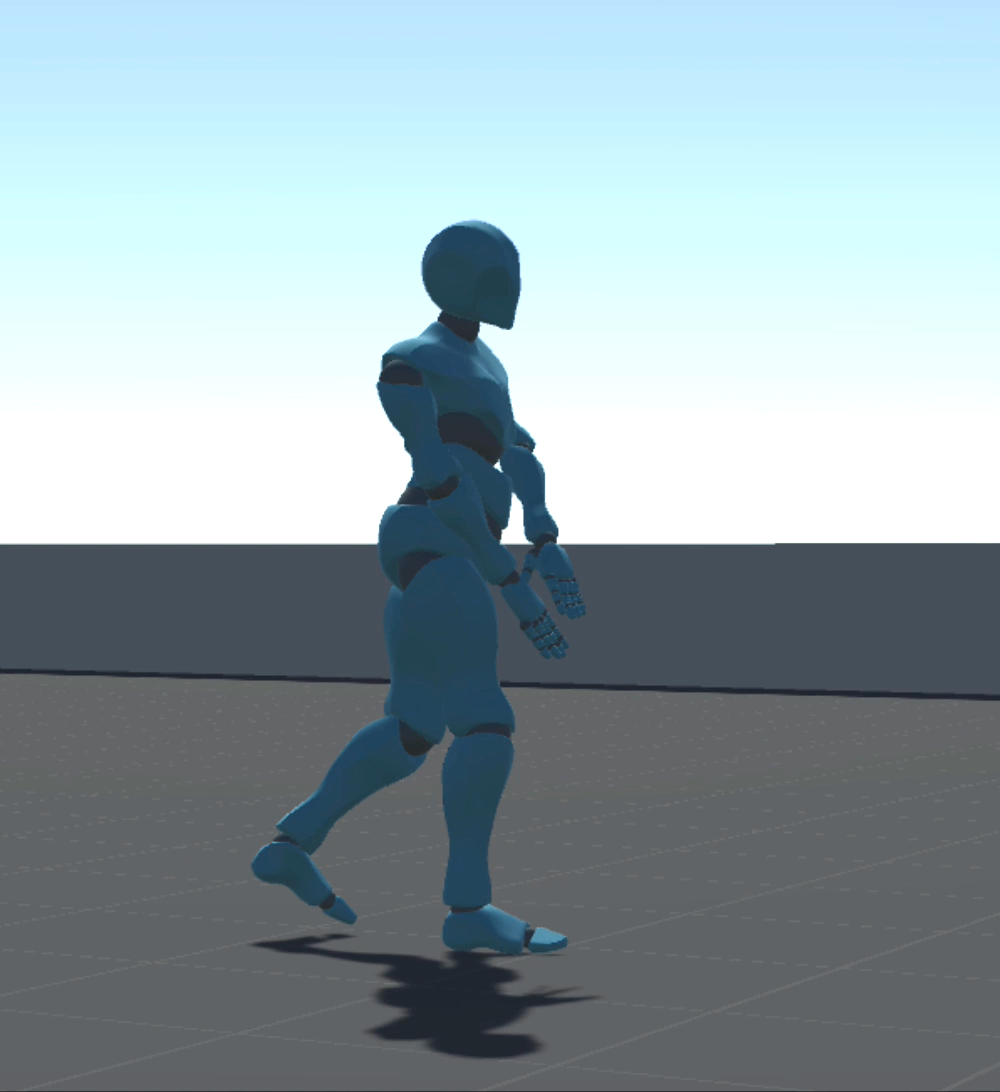
\includegraphics[width=0.27\textwidth]{img/charakter_mixamo_laufen_energiespar1} & 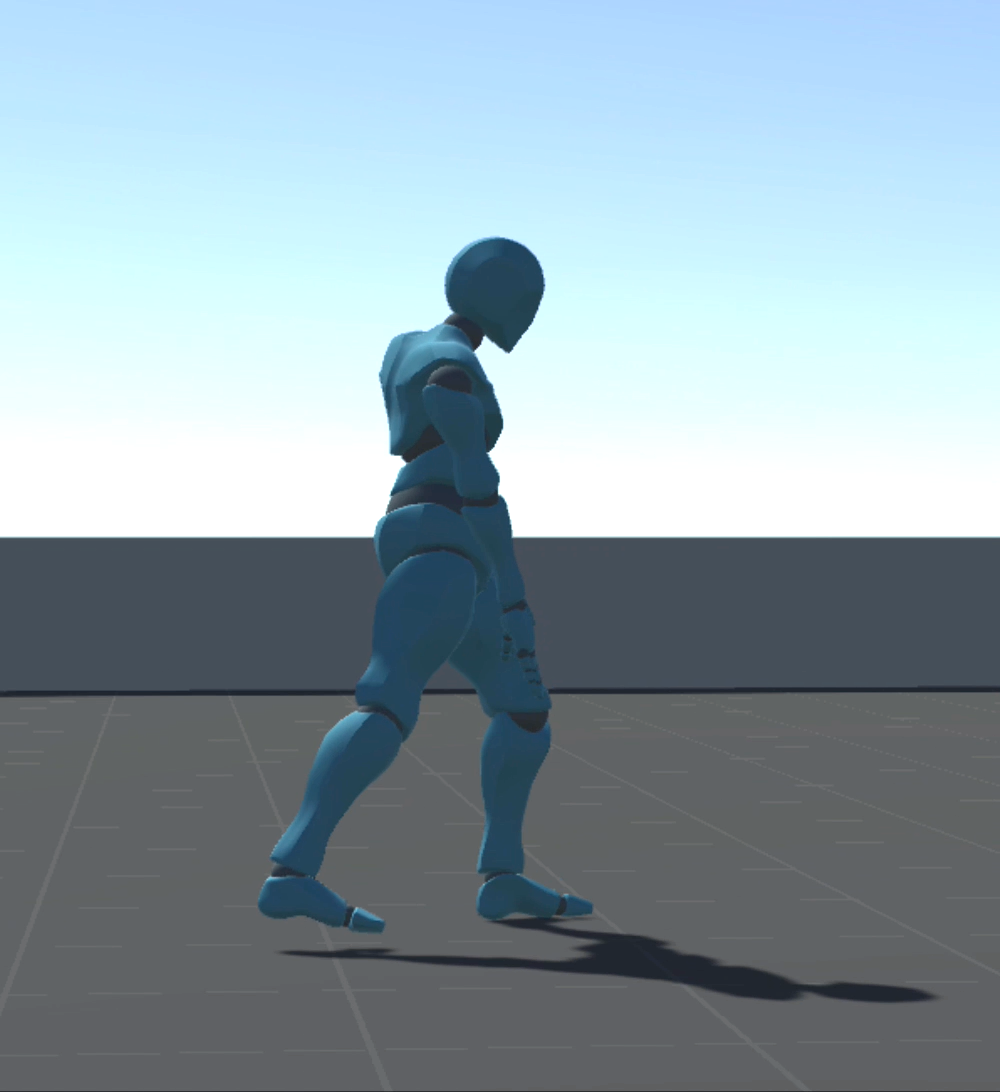
\includegraphics[width=0.27\textwidth]{img/charakter_mixamo_laufen_energiespar2}  & 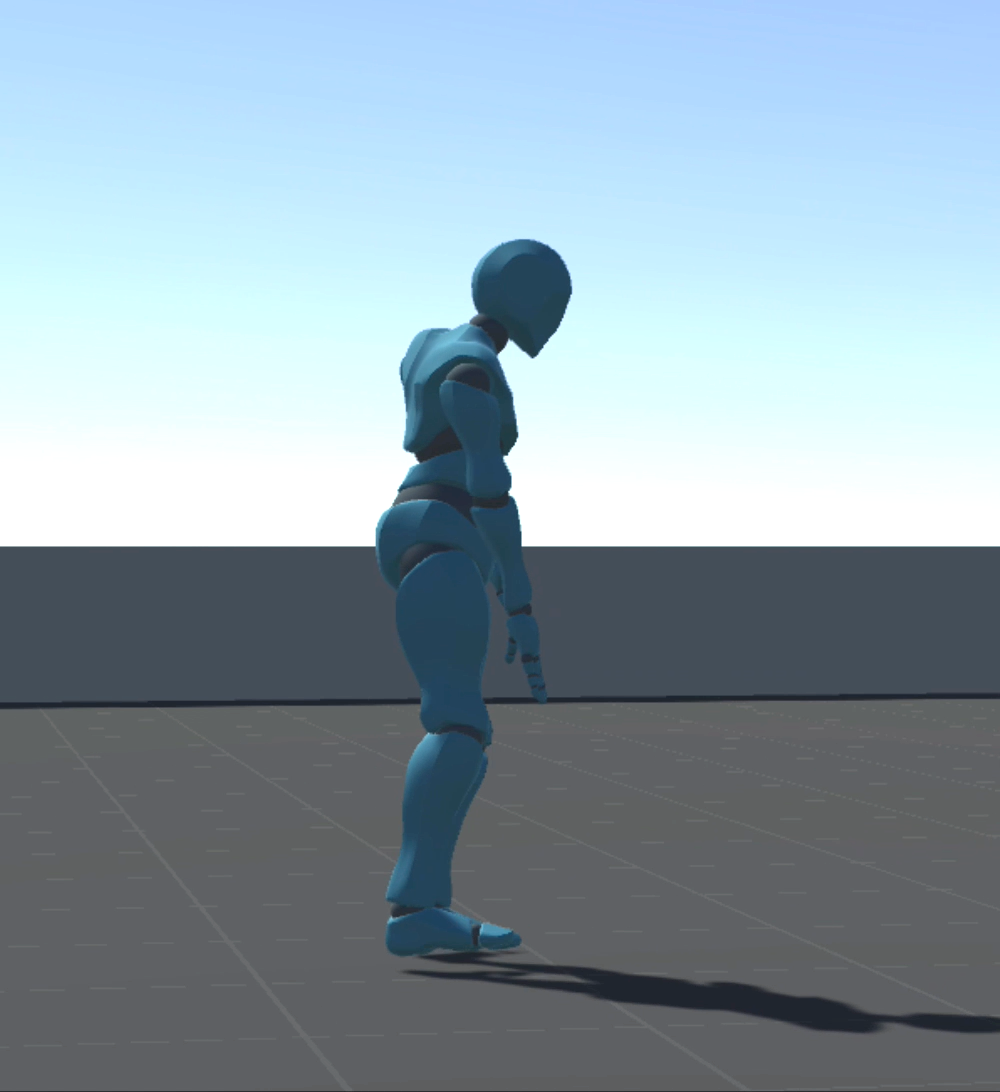
\includegraphics[width=0.27\textwidth]{img/charakter_mixamo_laufen_energiespar3} \\
    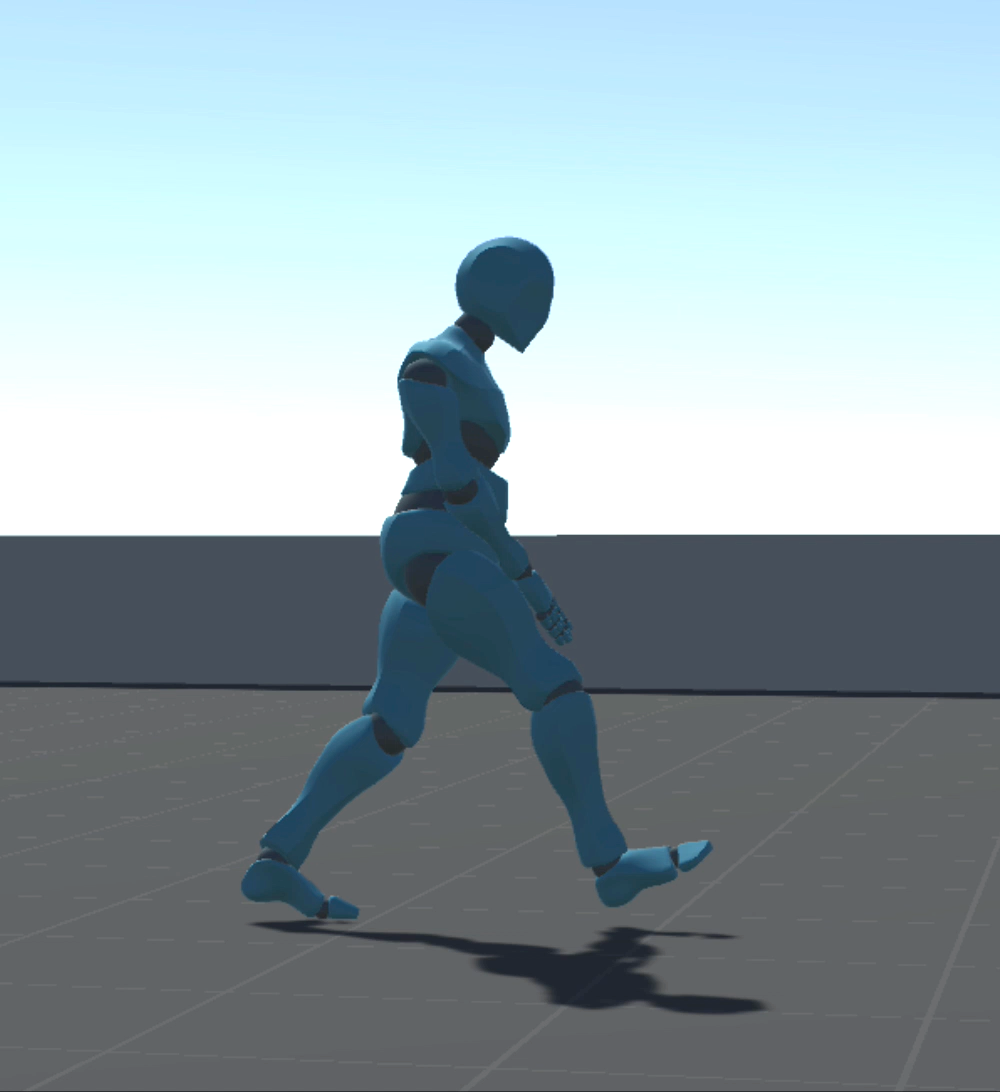
\includegraphics[width=0.27\textwidth]{img/charakter_mixamo_laufen_energiespar4}  & 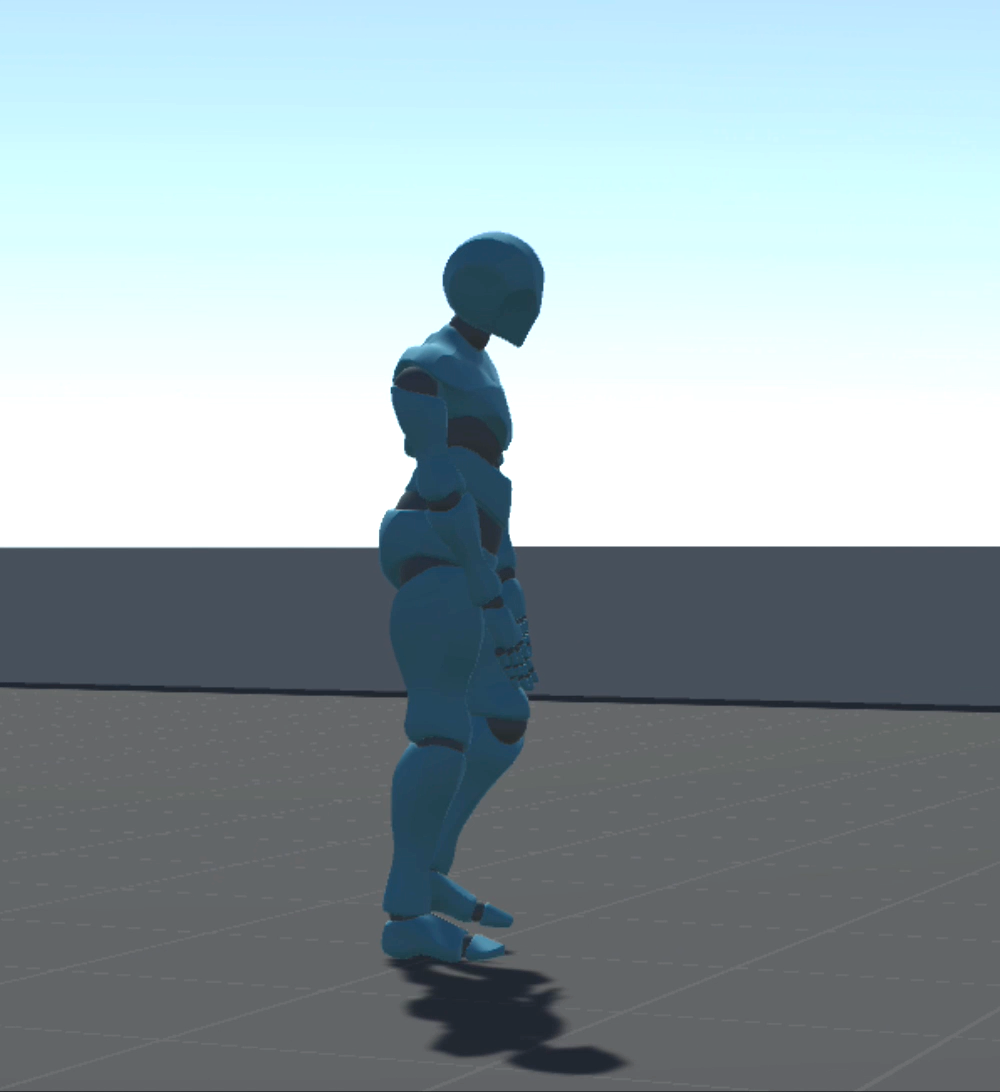
\includegraphics[width=0.27\textwidth]{img/charakter_mixamo_laufen_energiespar5}  & 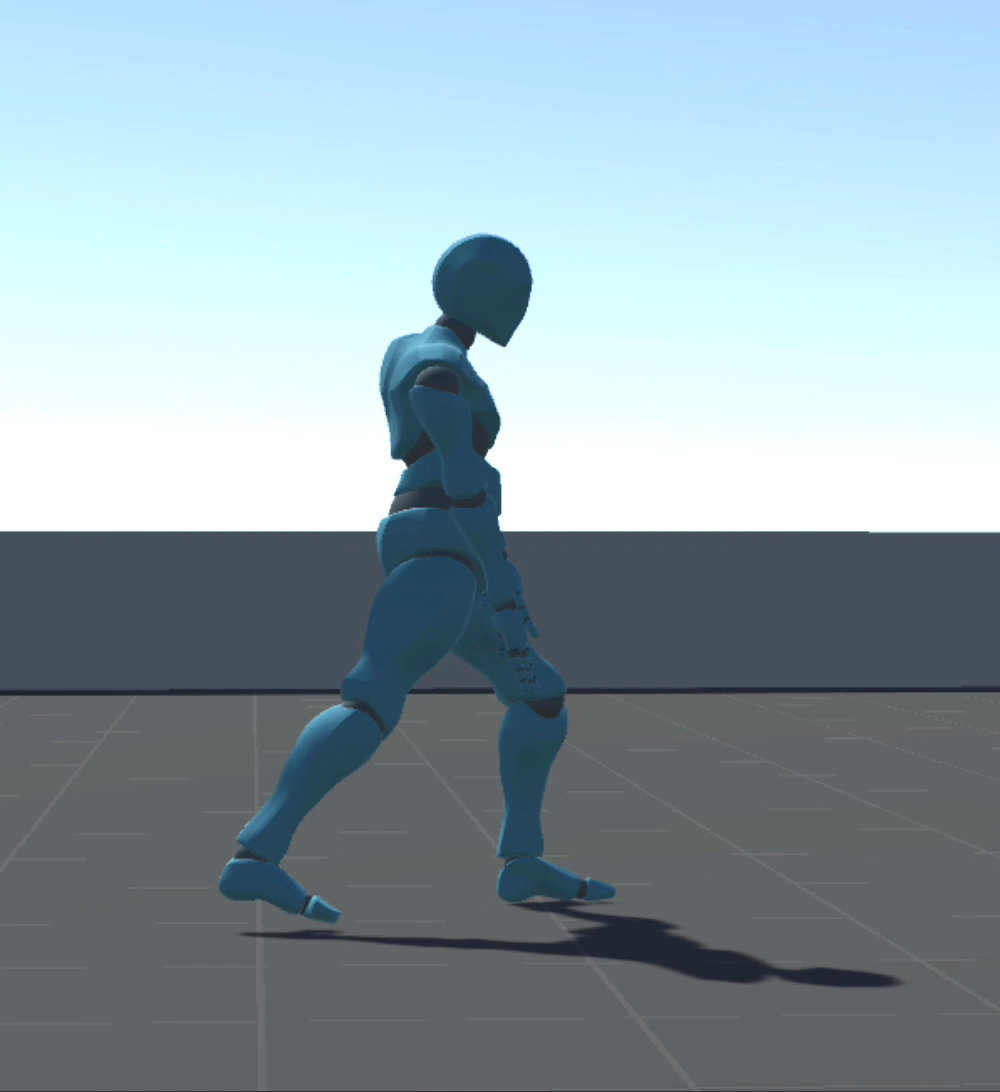
\includegraphics[width=0.27\textwidth]{img/charakter_mixamo_laufen_energiespar6} \\
  \end{tabular}
  \caption{Mixamo Versuch 12 Gangbild}
  \label{fig:mixamo_versuch12_gangbild}
\end{figure}

\subsection{Armpendel}
Die Arme sind für eine natürliche Gehbewegung unabdinglich. Ein gesunder Mensch bewegt die Arme beim gehen gegensätzlich zu den Beinen. Einige Vermutungen, warum der Mensch dieses Verhalten zeigt, sind die Verbesserung der Stabilität, Energieminimierung oder die Abstammung von Vorfahren, welche die Arme aktiv beim Fortbewegen einsetzten.\cite{meyns2013and}

Der Grund ist für die Entwicklung eines natürlichen Charakterkontrollers jedoch zweitrangig. Durch die vereinfachte physikalische Darstellung muss das für Menschen natürliche Verhalten teilweise über Umwege antrainiert werden. Um die Arme während des Laufens gegensätzlich zu den Beinen zu schwingen, wird die Verwendung einer weiteren Bestrafung getestet. Für die Bestrafung wird die Distanz der Hände, sowie Hüfte zum Ziel berechnet. Abhängig von der führenden Seite (Bein vorne) werden die Werte so aufsummiert, dass bei korrekter Armorientierung ein positiver Wert und gleicherweise bei falscher Armorientierung ein negativer Wert herauskommt. Ist das linke Bein vorne, sieht die Berechnung wie folgt aus: $(hüftdistanz - rechteHandDistanz) + (linkeHandDistanz - hüftDistanz)$ ist das rechte Bein vorne, werden die Hand Distanzen vertauscht und man erhält $(hüftdistanz - linkeHandDistanz) + (rechteHandDistanz - hüftDistanz)$.

\begin{figure}[H]
  \centering  
    \begin{subfigure}{.49\textwidth}
      \centering  
      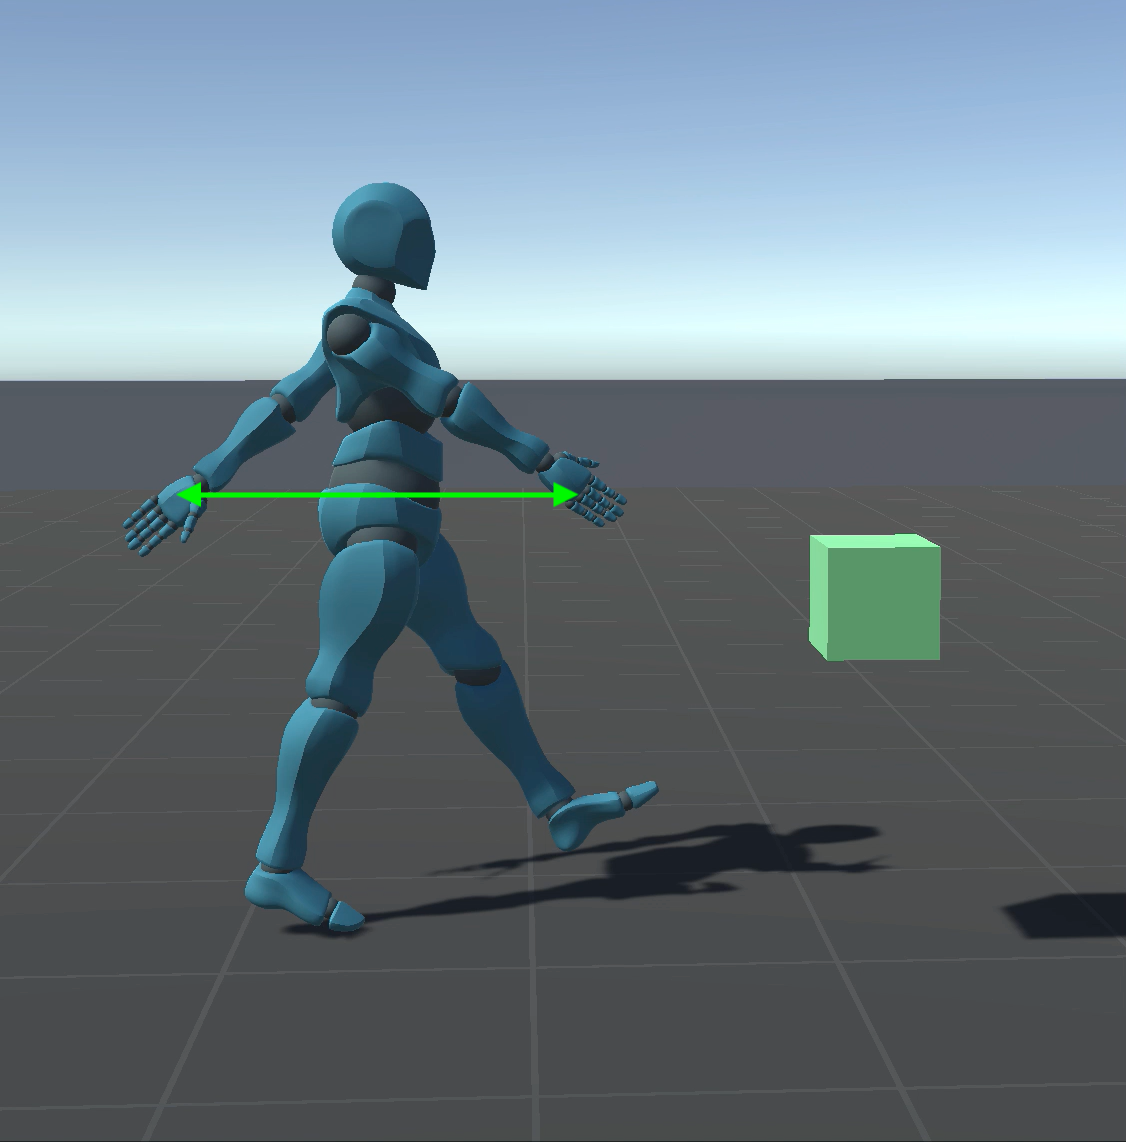
\includegraphics[width=\textwidth]{img/hand_pendel_gut}
      \caption{Richtige Armpendel Richtung (Distanz positiv)}
      \label{fig:hand_pendel_gut}
    \end{subfigure}
    \begin{subfigure}{.49\textwidth}
      \centering  
      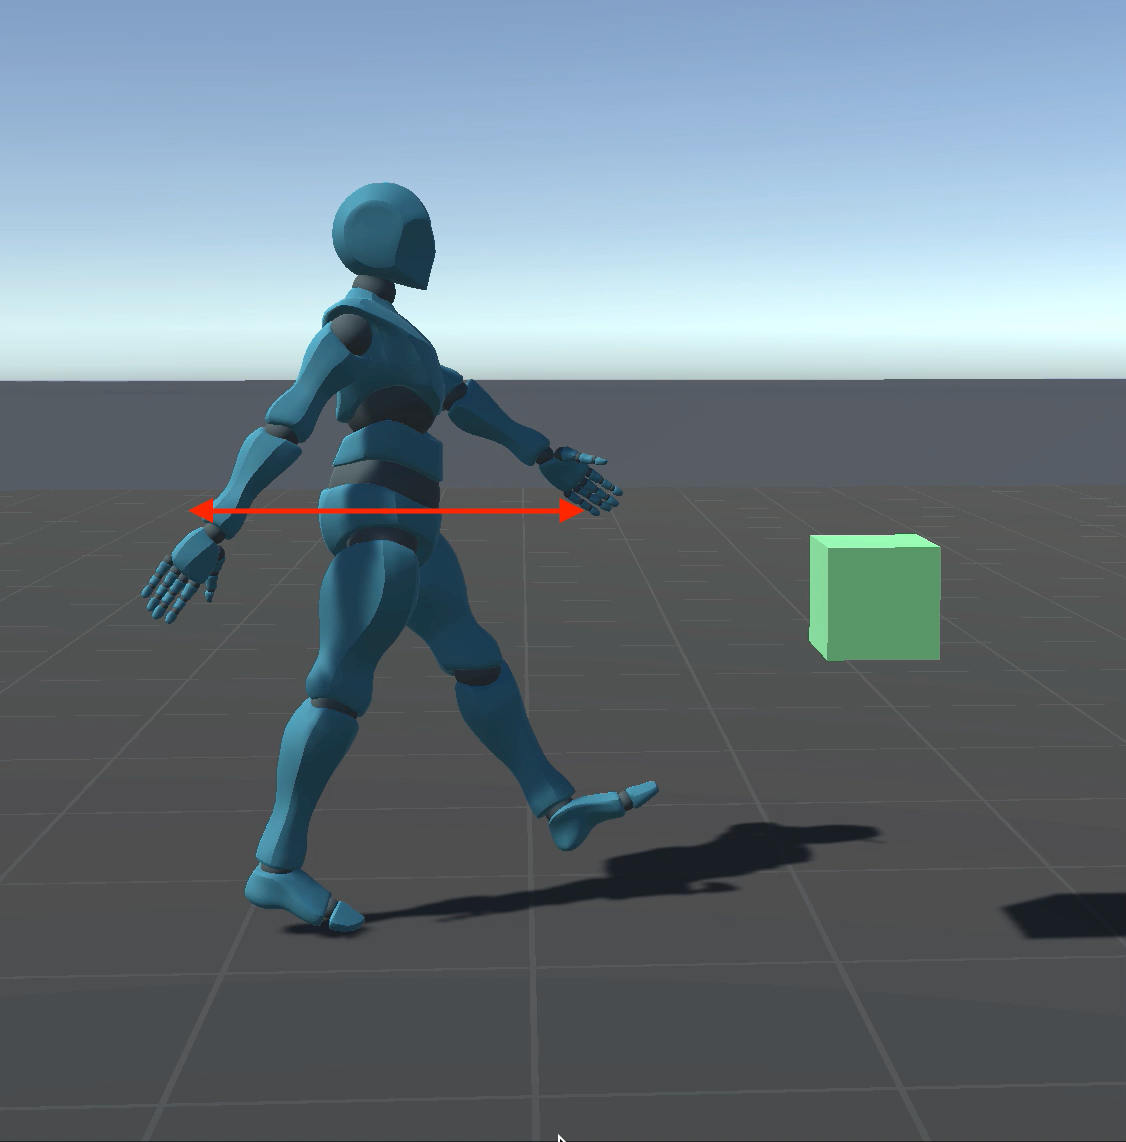
\includegraphics[width=\textwidth]{img/hand_pendel_schlecht}
      \caption{Falsche Armpendel Richtung (Distanz negativ)}
      \label{fig:hand_pendel_schlecht}
    \end{subfigure}
  \caption{Pendelsumme Distanz veranschaulichung}
  \label{fig:pendelsumme_distanz}
\end{figure}

Anschließend wird die Distanz mit einer Clip ähnlichen Funktion (siehe Abbildung \ref{fig:plot_hand_pendel}) auf einen Bereich von -1 bis 1 beschränkt, abschließend werden die Werte auf einen Bereich von -1 bis 0 skaliert.

\begin{figure}[H]
  \centering  
  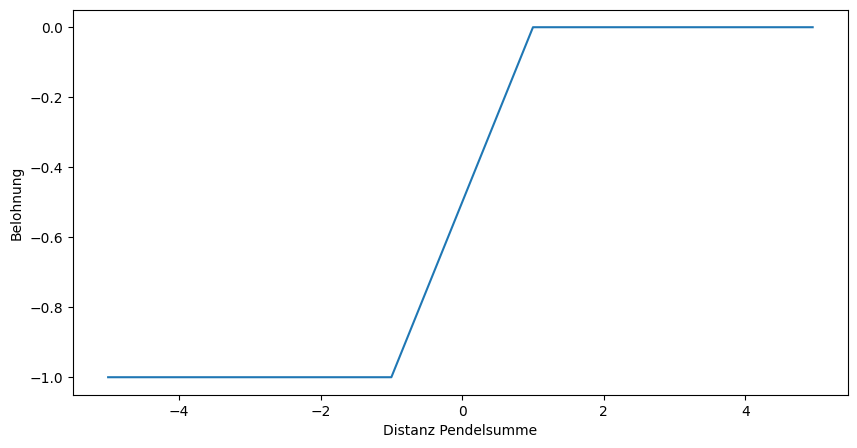
\includegraphics[width=\textwidth]{img/plot_hand_pendel}
  \caption{Armpendel Bestrafung}
  \label{fig:plot_hand_pendel}
\end{figure}

Die neu eingeführte Armpendel Bestrafung hat nicht die erwarteten Ergebnisse erzielt. Zu Beginn des Trainings dominiert die Bestrafung so stark mit -0,48 Punkten pro Trainingsschritt. Das der Läufer sich entscheidet nur diese Bestrafung zu optimieren und gleichzeitig so schnell wie möglich das frühe Stop auszulösen, um zusätzliche Bestrafung zu verhindern. Um zu evaluieren ob die entwickelte Belohnungsfunktion das gewollte Verhalten verstärkt, muss hier ein Training mit weniger starken Bestrafungen durchgeführt werden.

\subsection{Imitationslernen}
Imitationslernen ist eine weit verbreitete Technik, um Agenten im verstärkenden Lernen ein bestehendes Verhalten anhand von Aufzeichnungen anzutrainieren. Ein Vorteil des Imitationslernens besteht darin, dass natürliche Verhaltensmuster aus der Referenz übernommen werden und somit weniger spezialisierte Belohnungen erforderlich sind. Als Referenz für die Steuerung menschlicher Charaktere werden Bewegungsaufnahmen von Menschen verwendet. Unity ML-Agents bietet für das Imitationslernen zwei Algorithmen an: Behavioral Cloning und Generative Adversarial Imitation Learning. Beide verwenden als Referenz eine aufgenommene Demonstration. Zum Aufnehmen einer Demonstration existiert die Demonstration Recorder Komponente, die auf ein Objekt mit Agent hinzugefügt wird. Anschließend kann das heuristische Verhalten des Agenten aufgezeichnet werden. Im Fall der Läufer-Trainingsumgebung ist es jedoch schwierig, ein solches Verhalten zu entwickeln, da zusätzlich zu den Gelenkrotationen, die aus Bewegungsaufnahmen entnommen werden können, auch die Gelenkstärke benötigt wird. Aufgrund dieser Anforderungen sind die von Unity ML-Agents verfügbaren Systeme für das Imitationslernen in diesem Fall nicht geeignet. Daher wurde das Imitationslernen basierend auf den in der Arbeit \grqq{}DeepMimic: Example-Guided Deep Reinforcement Learning of Physics-Based Character Skills\grqq{} entwickelten Imitationsbelohnungsfunktionen getestet.\cite{peng2018deepmimic} Als Referenzbewegung werden Motion Capture Daten aus der \grqq{}SFU Motion Capture Database\grqq{} genutzt.\cite{sfu-motion-capture}

Zu Beginn einer Trainingsepisode wurde die Referenzanimation zurückgesetzt und der Läufer auf die gleiche Startpose gesetzt. Der Agent erhält zusätzlich zu seiner normalen Beobachtung auch eine Phasenvariable, die die aktuelle Phase der Animation widerspiegelt. Es wurde untersucht, wie sich die Kombination der Körperhaltungsbelohnung (Posereward) aus dem Deep Mimic Artikel mit den Walker Demo Belohnungen auf das Verhalten auswirkt. Die Körperhaltungsbelohnung belohnt die Übereinstimmung der relativen Körperteilrotationen und ist somit positionsunabhängig. Da jedoch die Hüfte bzw. das Hauptkörperteil eines Charakters keine Referenz hat, zu der diese Rotation relativ bestimmt werden kann, wurde eine Ausnahmeregel für die Hüfte entwickelt, die nur die Rotation in zwei Richtungen vergleicht: die X- und Z-Rotation. Die Rotation um die Y-Achse wird ignoriert, um unterschiedliche Orientierungen des Körpers und damit unterschiedliche Zielrichtungen zuzulassen, ohne diese zu bestrafen. Der Läufer entwickelte ein rückwärts übergebeugtes Gehverhalten (siehe Abbildung \ref{fig:charakter_mixamo_imitation}), es ist unklar, ob der Läufer die Referenzbewegung teilweise imitiert hat. Der Auslöser für das merkwürdige Gangbild ist ebenfalls nicht eindeutig. Eine mögliche Ursache könnte ein Fehler im Vergleich der Hüftrotation sein.

\begin{figure}[H]
  \centering  
  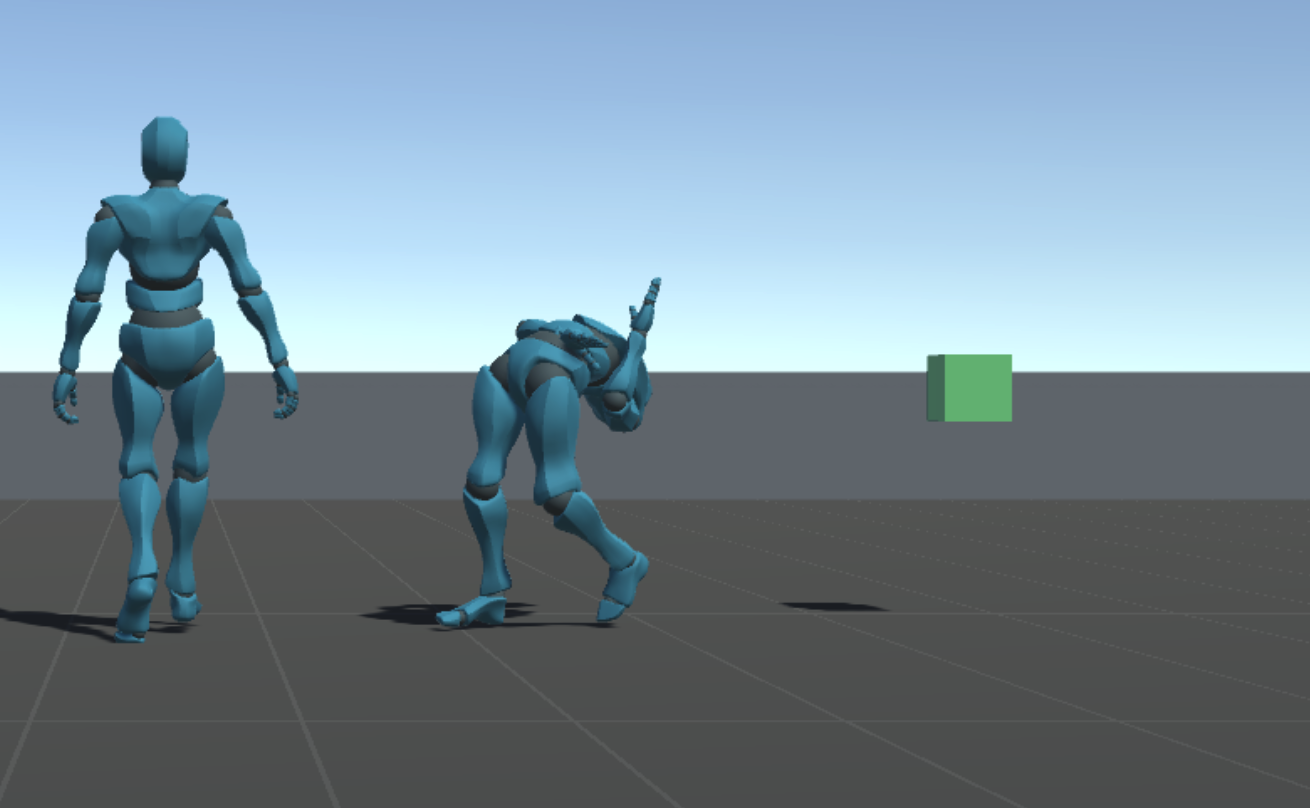
\includegraphics[width=0.9\textwidth]{img/charakter_mixamo_imitation}
  \caption{Mixamo mit Walker- und Körperhaltungbelohnung}
  \label{fig:charakter_mixamo_imitation}
\end{figure}